\documentclass[a4paper,twocolumn,10pt]{ltjsarticle}

\usepackage{geometry}
\geometry{top=20mm, bottom=24mm, left=23mm, right=23mm}

\usepackage{graphicx}

\makeatletter
  % maketitle
  \def\@maketitle{%
    \newpage
    \begin{center}%
     %和文題名
     {\Large \textbf{\@title} \par}%
     \vskip 9pt
     %和文著者
     {\large \lineskip .0em
     \begin{tabular}[t]{c}%
      \@author
     \end{tabular} \par}%
     %英文題名
     \vskip 1.5em
     {\Large \textbf{\etitle@etitle} \par}%
     \vskip 0.5em
     %英文著者
     {\large \lineskip .0em
     \begin{tabular}[t]{c}%
      \etitle@eauthor
     \end{tabular} \par}%
     \vskip 0.5em
    \end{center}%
    \par\vskip 1.5em
    \ifvoid\@abstractbox\else\centerline{\box\@abstractbox}\vskip1.5em\fi
    }
  % \title \author は既存のマクロを利用 \@title \author に値がセットされる.
  \newcommand{\etitle@etitle}{}
  \newcommand{\etitle@eauthor}{}
  \newcommand{\affiliation}[1]{\renewcommand{\etitle@affiliation}{#1}}
  \newcommand{\etitle}[1]{\renewcommand{\etitle@etitle}{#1}}
  \newcommand{\eauthor}[1]{\renewcommand{\etitle@eauthor}{#1}}
\makeatother

% !!!重要!!! ファイル先頭からこの行までの間は改変しないこと.

% 必要に応じて適宜パッケージを追加
% 例:特殊な数学記号を利用する→ \usepackage{amsmath} など
\usepackage{url}     % URLを \url{} で括ると見やすくなる

% 和文題名
\title{宮下ゼミ卒業論文テンプレート2021}
% 和文著者
\author{京都女子大学 現代社会学部 現代社会学科 宮下ゼミ\\
18241000 東山 京子}
% 英文題名
\etitle{Manuscript Template for Graduation Thesis in Miyashita Lab 2021}
% 英文著者. 和文所属と同様です
\eauthor{Miyashita Lab., Faculty for the Contemporary Society, Kyoto Women's University\\
18241000 Higashiyama Kyoko}

% 論文の概要
\begin{abstract}
これは宮下ゼミの学生向けに書かれた卒業論文のテンプレートである.
ここには卒業論文の概要(論文内容を簡潔にまとめたもの)を書く.
研究の動機や背景,問題,解決手法,結論などを簡潔にまとめる(参考文献番号は不要).
概要を読めば論文内容がだいたい示されているようにすることが重要である(もともと「概要」とはそのようなものである).
文章量は特に定めないが,だいたい4〜8行程度にすればバランスがよいと思われる.
\end{abstract}

\begin{document}
% \begin{document} 直後に \maketitle コマンドを置く
\maketitle

\section{はじめに}

これは京都女子大学現代社会学部宮下ゼミの学生向けに書かれた卒業論文テンプレートである.
宮下ゼミの学生はこの内容をよく理解し,すばらしい卒業論文を作成してもらいたい.

\section{卒業論文作成の流れ}

卒業論文は以下のように作成し,提出すること.

\subsection{論文の作成}

卒業論文は電子的な形態を第一とし,紙に印刷されたものは副次的なものとする.
つまり教務課に提出するものは第二形態であり,原本は飽くまでも電子ファイル(PDF形式)である.

卒業論文は,このファイルのように文書処理システム\LaTeX{}を利用して作成し,PDF形式で提出する.

\subsection{論文の提出}

卒業論文の「提出」は通常2つあるので注意されたい.
一方はゼミ内での提出であり,他方は教務課への提出である.
この両方が必要である.

前者では,PDF形式のファイルを教員が指定した方法でアップロードする.
京女ポータル内LMSまたはMicrosoft Teamsの演習VIチャネルに「卒業論文」という課題が作成され,そこへアップロードすることになるが,具体的な提出方法については演習VIで伝える.

後者は,印刷された原稿を教務課窓口へ提出するのが通例である\footnote{今後社会情勢の変化により提出方法が変更される可能性があるので京女ポータルのお知らせに注意すること.}.
この際,印刷した原稿は左上をホチキス等で綴じること.

どちらも2022年1月17日17時が〆切である.
特に教務課への提出は〆切に遅れると取り返しがつかないので充分注意すること.

\section{論文作成要領}

卒業論文は電子的な媒体で読む(例えばPCやタブレットの画面で閲覧する)のに適するよう作成し,PDF形式のファイルで提出する.
PDF形式であれば文字はもちろんのこと図なども鮮明に表示/印刷されることが期待できるからである.

\subsection{論文の書式}

読みやすく明瞭かつ正確な原稿とするために,以下の指示にしたがって執筆する.

\begin{itemize}
 \item 原稿はA4判2段組で4ページ以上8ページ以下とする.
 \item ページ数は,わかりやすさを損ねない範囲でできるだけ少なくする.
 \item 長大なプログラムリストなどが必要不可欠な場合は,付録として原稿の末尾に付す(これはページ数に含めない).
 \item 先頭ページ上部に題名,所属,著者名を日本語と英語で記載する.
 \item 本文の文字の大きさは10ポイントとする(図表中の文字も原則として本文と同程度の大きさとする).
 \item 本文は日本語または英語で記述する.
 \item 本文は読みやすいようにいくつかの節\footnote{大抵の場合,「はじめに」で始まり,本論を述べ,「おわりに」で終わる.その後,謝辞と参考文献が続く.}や段落に分け,明瞭簡潔な記述を心がける.
 \item 本文の文章は常体で記述し,句読点はコンマ「,」とピリオド「.」(どちらも全角)とする.
 \item 著者自身を表したいときは「著者は〜」などとし,「私」は用いない.
 \item 文章や図表などを引用したり参考にしたりする際は出典を明示し,著作権を侵害しないよう注意する.
 \item お世話になった人には謝辞を述べる.
\end{itemize}

\subsection{PDFファイルの作成}

卒業論文として提出できるファイル形式はPDFだけである.
その際,以下のことに注する.

\begin{itemize}
 \item ファイル名には拡張子({\tt .pdf})を必ず付すこと(ファイル名そのものは何でも構わない).
 \item 図として画像を利用する場合は解像度を適切に設定する(少なくとも150dpi程度以上).
 \item 編集不可・印刷不可などのセキュリティ設定を施さない.
\end{itemize}

\section{図表の書き方}

図表は本文中に埋め込み,番号とキャプションを付す.
図表の配置と番号付けは\LaTeX{}により自動的に行われるのでそれに任せる.
キャプションはその図表を表す端的なものとする.
図表は必ず本文中から参照するものとし,その際は図表の番号で参照する.

以下,図の例を図\ref{fig:graphs}に示す.
図は中央寄せ(センタリング)とし,図のキャプションは図の直下に記述する.

\begin{figure}[htb]
 \begin{center}
  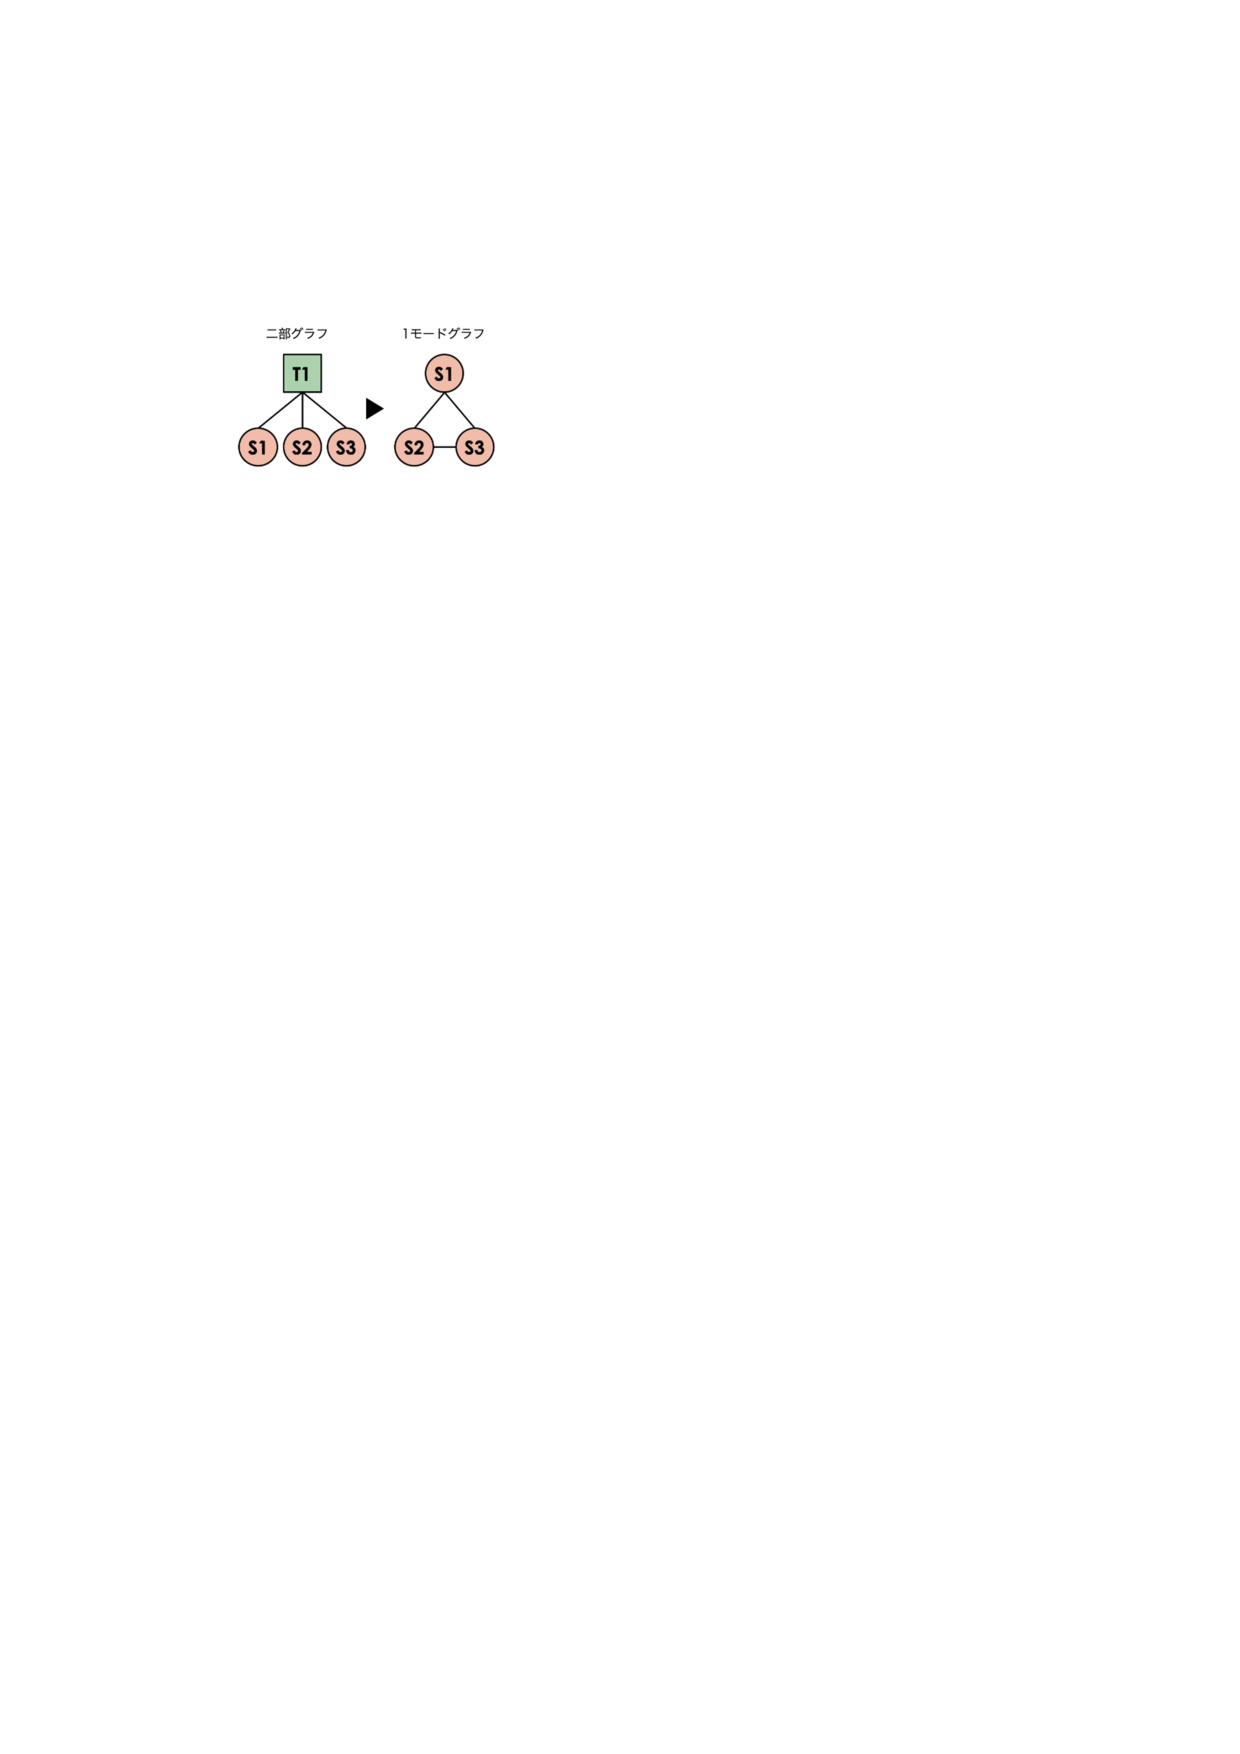
\includegraphics{graphs.pdf}
  \caption{2部グラフから1モードグラフへの変換}
  \label{fig:graphs}
 \end{center}
\end{figure}

また,表の例を表\ref{tab:competency}に示す.
表もセンタリングし,表のキャプションは表の直上に記述する.

\begin{table}[htb]
 \begin{center}
  \caption{コンピテンシーディクショナリの項目数}
  \label{tab:competency}
  \begin{tabular}{cccc}
   \hline
   名称 & タスク & スキル & 関連知識\\
   \hline
   項目数 & 639 & 491 & 8843\\
   \hline
  \end{tabular}
 \end{center}
\end{table}

\section{参考文献の書き方}

参考文献は論文での出現順に記載し,巻末に一覧を掲載する.
その際,雑誌の場合\cite{refjournal1,refjournal2}と書籍の場合\cite{refbook1,refbook2},WWWページの場合\cite{refwww}それぞれ以下の通りに記述し,この文章のように参考文献を参照している箇所に参考文献番号を記載する.

\begin{itemize}
 \item 雑誌の場合:著者名,タイトル,雑誌名,巻,号,ページ,発行年.
 \item 書籍の場合:著者名,書名,参照ページ(あれば),発行所,発行年.
 \item WWWの場合:タイトル,URL,アクセス日.
\end{itemize}

\section{おわりに}

京都女子大学現代社会学部宮下ゼミの学生向けに,卒業論文のテンプレートを示した.
すばらしい卒業論文が作成されることを期待している.

\section*{謝辞}

研究を進めたり卒論を作成したりしたときにお世話になった人(指導教員,友人,知人,親戚等)がいれば,この節に具体的に記して謝意を述べる.
この節の文章は敬体でも良い.
例えば「○○教授には卒業論文作成全般にわたりご指導いただきました.深く感謝します.」
「○○氏には○○に関する重要な示唆をいただきました.感謝します.」
「○○についての有用なデータをご提供いただいた○○氏に感謝します.」など.

\begin{thebibliography}{99}
 \bibitem{refjournal1} 宮下健輔,水野義之,京都女子大学における全学情報教育とそれを支える情報システムの変遷に関する考察,情報処理学会論文誌,Vol.53,No.3,pp. 997--1004,2012.
 \bibitem{refjournal2} Kensuke Miyashita, Yuki Maruno, Campus Wireless LAN Usage Analysis and Its Applications, NEURAL INFORMATION PROCESSING, ICONIP 2016, PT I, pp. 563--569, 2016.
 \bibitem{refbook1} 河野哲也,レポート・論文の書き方入門 第4版,慶応義塾大学出版会,2018.
 \bibitem{refbook2} 福地健太郎,園山隆輔,理工系のためのよい文章の書き方,翔泳社,2019.
 \bibitem{refwww} Overleaf, {\tt https://ja.overleaf.com/}, 2021年7月26日アクセス.
\end{thebibliography}
\end{document}
